\chapter{Introduction}
Many patients suffer with a chronic illness or disorder (e.g. chronic pain\cite{chronic_pain}, migraines\cite{migrane}, anxiety\cite{anxiety}, panic attacks\cite{panic_attack} or PTSD\cite{ptsd_stats} just to name a few). To better treat these illnesses it is important to figure out what can trigger an episode (episode meaning the negative effect of the illness, e.g. a headache if suffering from migraines), this can be done by tracking when and where episodes happen in order to look for patterns. The problem with these illnesses is that their episodes require to be tracked manually by the patient, since no technology yet exist that can measure these on its own. Providing a way to accurately gather when patients are experiencing the effects of their conditions would be valuable information that could help treat their illness, or at least help to prevent scenarios that can trigger episodes. 

Manual tracking has traditionally been done with pen and paper, either in the moment or as a daily diary where the patient by the end of the day will log their experiences for the whole day. The problem with daily diaries are that they introduce memory recall bias\cite{recall_bias}, which causes issues with the reliability of data reported by patients. Thus it is important to gather data on patients when they are exposed the effects of their illness. In recent times different different solutions have been created trying to improve this, using an app on either a smartphone or smartwatch eliminates memory recall bias by enabling the patient to log what they are experiencing in the moment. At first this seems like an ideal solution, but one problem becomes apparent and that is burden of use. Using a tracking app on a smartphone requires the user to get the smartphone out of their pocket, turn it on, unlock it, find the app, open it and then log the event. While this is a bit easier using a smartwatch since it in it natures is always at your wrist, it still requires at least a couple of interactions and requires the user's full attention while interacting with the smartwatch. It is of great importance to minimize the burden of logging experiences, and often the simplest solutions are shown to be the most effective.

An example has been a \say{smartbutton} which is a wristband device equipped with a single button, pressing it will log a single time stamp\cite{eg}. The interaction burden with such a device is very minimal, and it doesn't require the user's full attention, since it can be done whit out looking at the device. The downside of this solution is that it only allow to log when an event occurred and not the severeness. Another problem is how to measure and compare psychological events, in the medical field a Visual Analogue Scale (VAS)\ref{real_vas} is used to measure such events by letting the patient rate the experience on a continuous scale from 0 to 10. The meaning of the scale is then described to fit the domain, most used is the pain scale as seen in Figure \ref{real_vas}, where 0 is no pain and 10 is the worst imaginably levels of pain. The VAS can easily be used in many other domains simply by changing the explanation for the scale, for example to use with panic attacks 0 would be no panic attack and 10 would be worst imaginably panic attack.

\begin{figure}[h!]
    \centering
    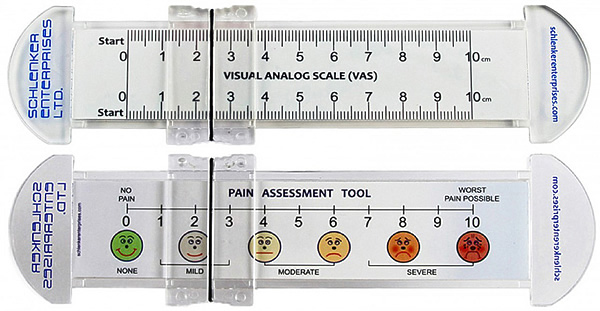
\includegraphics[width=0.9\textwidth]{figures/real_vas.jpg}
    \caption{VAS Pain Scale Ruler\cite{real_vas}}
    \label{real_vas}
\end{figure}

The proposed solution shall allow users to track whenever they experience events related to their illness. It need to be simple to use in order to minimize the burden of use. It should be able to track the severeness of the events in a way that resembles a VAS. The solution proposed in this thesis will be to create a wristband device that using gestures will map the rotation of the wrist or the elevation of the arm to a 0-10 scale. When the button on the wristband is pressed it will log the information based on the gesture. A companion app will be created to collect the data from the device and display the results to the user.

\section{Thesis Goals}
In this thesis the design and implementation of a wristband device and companion app for manual collection of data on subjective experiences using a gesture based system will be described. It aims to minimize the burden compared to other solutions and it aims to be reliable. An experiment will be conducted in order to compare the performance of the wristband with a digital version of a VAS.

\section{Contributions}
The focus of this thesis has been to design, implement and test two gesture based input methods to track the severeness of psychological experiences. The work of this thesis has resulted in the following contributions:

\begin{enumerate}
    \item Designed a system for tracking psychological experiences and their severeness on a continuous scale
    \item Implemented said system using a wristband device and Android app
    \item Created a method to map gestures of wrist and arm orientation to a continuous scale
    \item Designed an experiment for comparing said gestures to a VAS
    \item Conducted said experiment which results demonstrated the reliability of the implemented system
    \item Stated further problems worth investigating and possible improvements to the gesture based input technique
\end{enumerate}


\section{Thesis Structure}
This thesis is structured as follows. Chapter \ref{related_ch} detail the some of the most related work and it relates to this thesis. Chapter \ref{anal_ch} analysis the key concepts for this thesis that will form the foundation for this thesis. Chapter \ref{design_ch} details the design process for creating the proposed solution. Chapter \ref{implem_ch} details the implementation of the designed solution. Chapter \ref{eks_ch} presents and details an experiment conducted in order to compare the proposed solution to a digital VAS. Chapter \ref{res_and_dis_ch} presents the results collected results and discusses their meaning. Chapter \ref{future_ch} describes potential future work that could improve both the designed solution and experiment. Finally Chapter \ref{con_ch} concludes the thesis.




